\documentclass[11pt,dvipsnames]{scrreprt}

\usepackage[utf8]{inputenc}
\usepackage[ngerman]{babel}
\usepackage{fullpage} 			% kleinere Ränder

\usepackage{comment} 			% für größere comments: \begin{comment} ... \end{comment}
\usepackage{lscape} 			%für landscape-format

% *** für eingefügte (pdf-)Grafiken
\usepackage[pdftex]{graphicx}
\usepackage{epstopdf}
\usepackage{epsfig}
%\pdfminorversion=6
% ***

\usepackage{float} 
\usepackage{enumerate} 			%für geschachtelte Aufzählungen

\linespread{1.25}
\usepackage{amsmath} 			%Matheformeln usw.
\usepackage{amssymb} 			%mathfrak

\usepackage[bookmarks=true]{hyperref} 	% hyperrefs aktivieren
\setcounter{secnumdepth}{3} 		%Numerierung bis Tiefe 3, also ab \paragraph ohne
\setcounter{tocdepth}{1}

\usepackage{multirow}	 		%für Multirow Tabellen
\usepackage{forloop,supertabular}	% mehrseitige Tabellen
\usepackage{tabularx}

\usepackage{chngcntr}  			%Nummerierung neu beginnen
%\counterwithout{figure}{chapter}

%Farben
\usepackage{xcolor}
\usepackage{tikz}
\usetikzlibrary{shapes,snakes}

\usepackage{multicol}
\usepackage{dirtree}
\usepackage{minitoc}



%*** title usw.
\title{Dokumentation \\
    zur Studienarbeit im Fach\\
Praktikum Softwareengineering\\
\vspace{1cm}
- Entwicklung einer Lernsoftware -\\
"myMemo"\\
\vspace{5cm}
}
\author{ von Susanne Kießling\\
\vspace{2cm}
    Dozent: Prof. Dr. Martin Thost}
\date{\today}


\begin{document}
\maketitle
\tableofcontents

\clearpage

\chapter{Anforderungen des Kunden}
Die Diakonie Hochfranken möchte das Angebot an Lernsoftware in ihren Kindergärten und Kindertagesstätten erweitern. Es soll eine Lernsoftware entwickelt werden, die Gedächtnistraining und die Erweiterung des Wortschatzes spielerisch umsetzt.

\section{Systemvoraussetzungen}
Aktuell verfügt der Kunde über Einzelplatz-PC's, die in den Jahren 2005 bis 2010 angeschafft wurden. Als Betriebssystem kommt Linux und Windows zum Einsatz.

\section{Zielgruppe}
Die Besucher der Einrichtung im Alter von fünf bis zehn Jahren bilden die Zielgruppe der Software. 


\clearpage
\chapter{Lastenheft}

\section{Zielbestimmung} %welche Ziele sollen mit dem Software-Produkt erreicht werden.
Mit der Lernsoftware wird die Möglichkeit geschaffen, das pädagogisch wertvolle Prinzip des klassischen Memory-Spiel auf eine digitale Plattform zu übertragen. Zusätzlich zum Gedächtnistraining trägt die Vokabelfunktion zur Erweiterung des Wortschatzes bei. Die Führung einer Highscore ermöglicht den Vergleich der erreichten Punkte und steigert die Motivation der Benutzer, eine bessere Platzierung zu erreichen. Das erhöht wiederum den Lerneffekt. Neben dem Spielen an sich wird der Umgang mit dem Computer spielerisch erlernt. Vor Spielbeginn sind Attribute festzulegen und Meldungen der Software zu beachten. Das schult zusätzlich Logik. Der 2-Player-Modus unterstützt außerdem die Kommunikation mit anderen Spielern.


\section{Produkteinsatz} %Anwendungsbereiche und Stakeholders werden genannt
Die Lernsoftware kommt in den Kindertagesstätten der Diakonie Hochfranken zum Einsatz. Anwender der Software sind Besucher der Kindertagesstätte im Alter von fünf bis zehn Jahren.

\section{Produktfunktionen} %Hauptfunktionen werden beschrieben, Stakeholdergruppen
%zugeordnet und in 10er-Schritten durchnummeriert (LF nn).

$\backslash$LF10$\backslash$ \hspace{15 mm}Spieler neu erstellen \\
$\backslash$LF11$\backslash$ \hspace{15 mm}Spieler laden\\ % prüfen, ob Spieler bereits vorhanden
$\backslash$LF12$\backslash$ \hspace{15 mm}Spielerdaten ändern\\ \\  % löschen, ändern usw.

\noindent$\backslash$LF20$\backslash$ \hspace{15 mm}Anzahl der Spieler wählen\\
\noindent$\backslash$LF30$\backslash$ \hspace{15 mm}Thema wählen\\
\noindent$\backslash$LF40$\backslash$ \hspace{15 mm}Spielfeldgröße wählen\\

%\noindent$\backslash$LF20$\backslash$ \hspace{15 mm}Spielkarten verwalten\\
%\noindent$\backslash$LF30$\backslash$ \hspace{15 mm}Spielfeld erzeugen\\
%\noindent$\backslash$LF40$\backslash$ \hspace{15 mm}Spielzüge verwalten\\

\noindent$\backslash$LF50$\backslash$ \hspace{15 mm}Spiel starten\\

\noindent $\backslash$LF60$\backslash$ \hspace{15 mm}Highscore anzeigen\\
$\backslash$LF61$\backslash$ \hspace{15 mm}Urkunde drucken\\

\noindent$\backslash$LF70$\backslash$ \hspace{15 mm} Vokabeltraining\\ \\
\noindent$\backslash$LF80$\backslash$ \hspace{15 mm}Audiodaten abspielen \\ 


\section{Produktdaten} %permanent gespeicherte Hauptdaten werden festgelegt und in
%10er-Schritten durchnummeriert (LD nn).
$\backslash$LD10$\backslash$ \hspace{15 mm}Spielerdaten \\ \\
\noindent $\backslash$LD20$\backslash$ \hspace{15 mm}Highscoredaten \\ \\

\section{Produktleistungen} % besondere Anforderungen an Hauptfunktionen oder Haupt-
%daten (Ausführungszeit, Datenumfang, ... ) werden aufgezählt (LL nn).

\section{Qualitätsanforderungen} % allgemeine Eigenschaften wie gute Zuverlässigkeit,
%hervorragende Benutzbarkeit, normale Effizienz, ... werden festgelegt.
Funktionalität:	\hspace{15 mm}		gut\\
Zuverlässigkeit:\hspace{15 mm}		sehr gut\\
Benutzbarkeit:	\hspace{15 mm}		gut\\
Effizienz:	\hspace{15 mm}		normal\\
Änderbarkeit:	\hspace{15 mm}		normal\\
Portierbarkeit:	\hspace{15 mm}		sehr gut\\
Spassfaktor:	\hspace{15 mm}		sehr gut\\
\section{Ergänzungen} % alles was nicht in obiges Schema passt und trotzdem wichtig ist.
Die Umsetzung der Software erfolgt in der Programmiersprache Java. Da der Kunde Linux und Windows als Betriebssystem einsetzt stellt dies die notwendige Portierbarkeit sicher.



\clearpage
\chapter{Aufwandskalkulation}
Die Aufwandskalkulation für die Planung, Analyse, Design, Konstruktion, Test und Einführung der Software wird anhand des Funktionspunktverfahren durchgeführt.

\clearpage
\section{Function Point Methode}
\begin{figure}[!h]
	\centering
    \includegraphics[width=15cm]{./FunctionPoint_filled.pdf}
	\label{layout_gesamt}
\end{figure}


\clearpage

\chapter{Use Case Diagramme}
Folgend wird die Software als Use Case Diagramme dargestellt. Use Case Diagramme stellen das System von außen dar. ............................................

\section{Spieler verwalten - $\backslash$LF10$\backslash$,$\backslash$LF11$\backslash$,$\backslash$LF12$\backslash$}
\begin{figure}[!h]
	\centering
    \includegraphics[width=\textwidth]{./SpielerVerwalten.png}
	\label{layout_gesamt}
\end{figure}

\clearpage
\section{Anzahl der Spieler wählen - $\backslash$LF20$\backslash$}
\begin{figure}[!h]
	\centering
    \includegraphics[width=\textwidth]{./AnzahlSpieler.png}
	\label{layout_gesamt}
\end{figure}

\clearpage
\section{Thema wählen - $\backslash$LF30$\backslash$}
\begin{figure}[!h]
	\centering
    \includegraphics[width=\textwidth]{./Thema.png}
    
	\label{layout_gesamt}
\end{figure}

\clearpage
\section{Spielfeldgröße wählen - $\backslash$LF40$\backslash$}
\begin{figure}[!h]
	\centering
    \includegraphics[width=\textwidth]{./Spielfeldgroesse.png}
	\label{layout_gesamt}
\end{figure}

\clearpage
\section{Spiel starten - $\backslash$LF50$\backslash$}
\begin{figure}[!h]
	\centering
    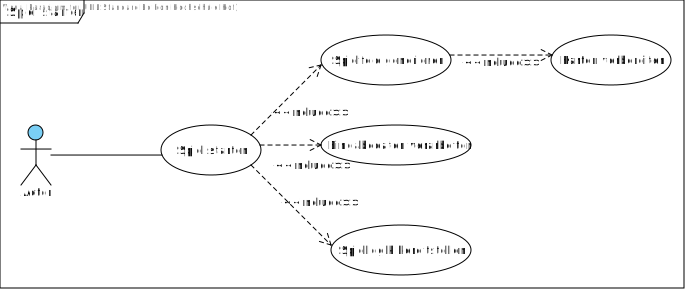
\includegraphics[width=\textwidth]{./SpielStarten.png}
	\label{layout_gesamt}
\end{figure}

\clearpage
\section{Highscore - $\backslash$LF60$\backslash$,$\backslash$LF61$\backslash$}
\begin{figure}[!h]
	\centering
    \includegraphics[width=\textwidth]{./Highscore.png}
	\label{layout_gesamt}
\end{figure}

\clearpage
\section{Vokabeltraining - $\backslash$LF70$\backslash$}
\begin{figure}[!h]
	\centering
    \includegraphics[width=\textwidth]{./SpielerVerwalten.png}
	\label{layout_gesamt}
\end{figure}

\clearpage
\section{Audiodaten abspielen - $\backslash$LF80$\backslash$}
\begin{figure}[!h]
	\centering
    \includegraphics[width=\textwidth]{./SpielerVerwalten.png}
	\label{layout_gesamt}
\end{figure}


\clearpage

\chapter{Use Case Beschreibungen}


\section{Spieler erstellen}
\begin{figure}[!h]
	\centering
    \includegraphics[width=\textwidth]{./ucbSpielerErstellen.png}
	\label{}
\end{figure}

\section{Abgleich mit Playerpool}
\begin{figure}[!h]
	\centering
    \includegraphics[width=\textwidth]{./ucbAbgleichPlayerpool.png}
	\label{}
\end{figure}


\clearpage
\section{Spieler laden}
\begin{figure}[!h]
	\centering
    \includegraphics[width=\textwidth]{./ucbSpielerLaden.png}
	\label{}
\end{figure}


\clearpage
\section{Spielmodus wählen}
\begin{figure}[!h]
	\centering
    \includegraphics[width=\textwidth]{./ucbSpielmodus.png}
	\label{}
\end{figure}

\clearpage
\section{Thema wählen}
\begin{figure}[!h]
	\centering
    \includegraphics[width=\textwidth]{./ucbThema.png}
	\label{}
\end{figure} 

\clearpage
\section{Spielfeldgröße wählen}
\begin{figure}[!h]
	\centering
    \includegraphics[width=\textwidth]{./ucbSpielfeldgroesse.png}
	\label{}
\end{figure}

\clearpage
\section{Spiel starten}
\begin{figure}[!h]
	\centering
    \includegraphics[width=\textwidth]{./ucbSpielStarten.png}
	\label{}
\end{figure}
\paragraph{Bemerkung: }Für die Include Use Cases 7 bis 9 werden keine Use Case Beschreibungen erstellt, weil es sich um Anwendungsfälle handeln, an denen ausschließlich das System beteiligt ist und interne Funktionen aufgerufen werden. Eine detailiertere Darstellung des Use Case ,,Spiel starten`` wird anhand von Sequenzdiagramm und Ablaufdiagramm bereitgestellt.

\clearpage
\section{Highscore anzeigen}
\begin{figure}[!h]
	\centering
    \includegraphics[width=\textwidth]{./ucbHighscore.png}
	\label{}
\end{figure}

\clearpage

\chapter{Projektplan}


\begin{figure}[!h]
	\centering
    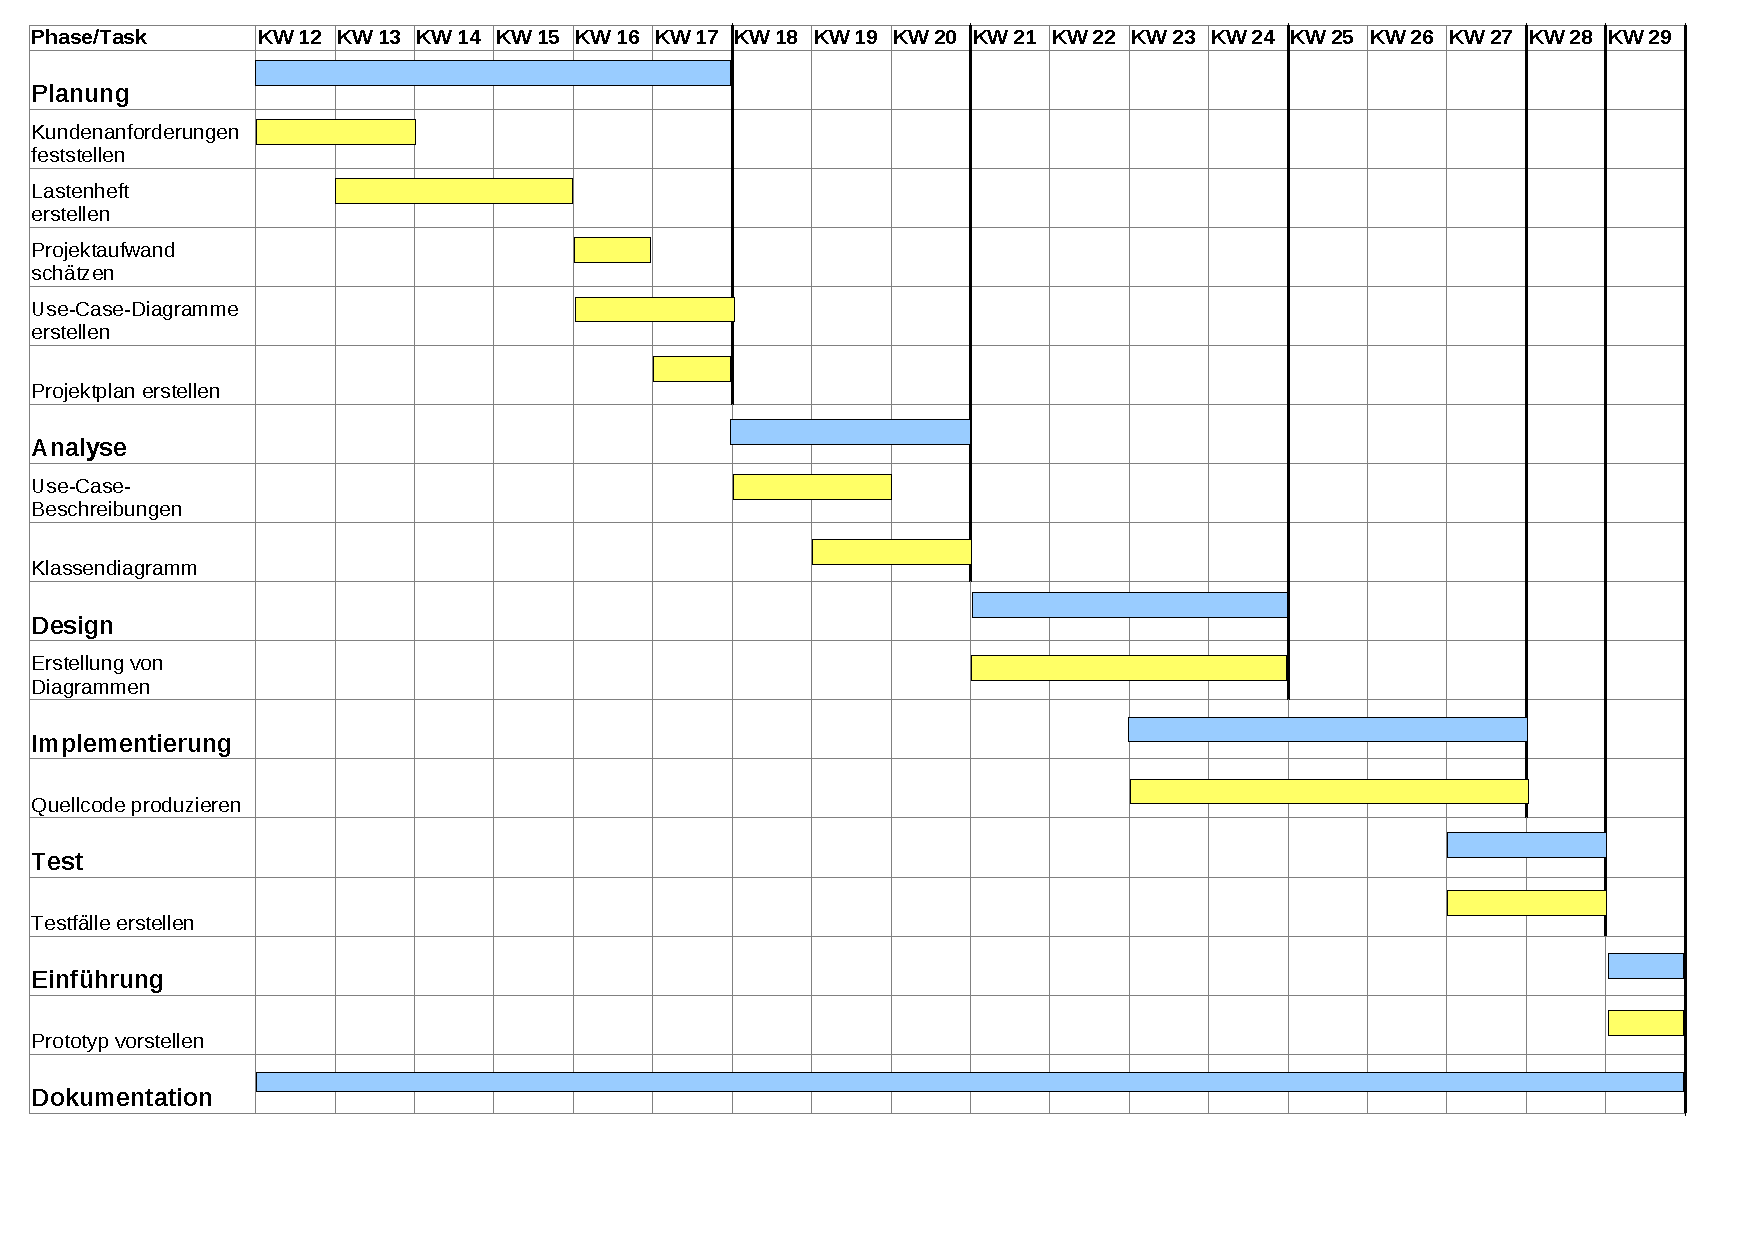
\includegraphics[width=\textwidth]{./projektplan.pdf}
	\label{layout_gesamt}
\end{figure}



\clearpage

\chapter{Klassendiagramm (vorläufig)}


\section{}


\section{}



\clearpage

\chapter{Sequenzdiagramme}
Sequenzdiagramme modellieren typische Szenarien eines Systems. Es wird die Kommunikation zwischen
Einheiten dargestellt.\\ \\
Folgende Use Cases wurden ausgewählt, um deren Kommunikation anhand von Sequenzdiagrammen darzustellen:\\
\begin{itemize}
  \item Spieler erstellen
  \item Spieler laden
  \item Spiel starten
\end{itemize}

\clearpage
\section{SD Spieler erstellen}
\begin{figure}[h!]
	\centering
    \includegraphics[width=13cm]{./SD_Spieler_erstellen.png}
	\label{layout_gesamt}
\end{figure}
\subsection{Beschreibung}
Der Benutzer wählt den Radio Button ,,Spieler erstellen''. Das Menue gibt das zugehörige Textfeld zur Eingabe des Namens frei. Nach Eingabe des Namens erfolgt ein Abgleich mit dem Playerpool, ob bereits ein Spieler unter diesem Namen gespeichert ist. Das Ergebnis wird zurück zur Klasse Menue geliefert. Ergibt die Prüfung, dass der Name noch nicht vorhanden ist, wir ein neues Objekt vom Typ Player erzeugt und anschließend dem Playerpool hinzugefügt. Ist der eingegebene Name bereits im Playerpool vorhanden, wird der Benutzer aufgefordert, einen anderen Namen einzugeben. Die Prüfung und Neueingabe erfolgt so lange, bis die Prüfung das Ergebnis = noch nicht im Playerpool vorhanden, liefert. Abschließend wird die nächste Menueseite angezeigt.

\clearpage
\section{SD Spieler laden}
\begin{figure}[h!]
	\centering
    \includegraphics[width=\textwidth]{./SD_Spieler_laden.png}
	\label{layout_gesamt}
\end{figure}
\subsection{Beschreibung}
Der Benutzer klickt den Radio Button ,,Spieler laden'' an. Daraufhin wird durch die Klasse Menue eine Liste der gespeicherten Spieler als Dropdown-Liste freigegeben. Daraus kann der Benutzer den gewünschten Namen wählen. Das Menue nimmt die Auswahl entgegen und holt sich den entsprechenden Player aus dem Playerpool. Anschließend wird die nächste Maske angezeigt.

\clearpage
\section{SD Spiel starten}
\begin{figure}[h!]
	\centering
    \includegraphics[width=15cm]{./SD_Spiel_starten.png}
	\label{layout_gesamt}
\end{figure}
\subsection{Beschreibung}
Der Benutzer drückt den Button ,,STARTEN``. Daraufhin werden von der Klasse Menue die Klassen GameField und GameController erstellt. Von GameField wird die Klasse Card erstellt. Hier werden die von der Klasse Menue übergebenen Parameter zum Erstellen des Spielfelds verarbeitet und die Karten gemischt. Anschließend wird dem Benutzer das Spielfeld angezeigt. Vom Benutzer wird eine Karte angeklickt. Dies wird in der Klasse Card aufgenommen und durch den Aufruf der Methode playGame() an den GameController weitergegeben. Der GameController ruft die Methode twoClicked() auf. Ist das Ergebnis true, wird die Methode compareCards() aufgerufen. Hat die Prüfung ergeben, dass die Karten übereinstimmen, werden die jeweiligen Karten mit der Methode setVisible(false) unsichtbar gemacht. Anschließend wird geprüft, ob das Spiel zu Ende ist. Trifft dies zu, wird die Methode checkWinner() aufgerufen und der hiermit ermittelte Gewinner dem Benutzer angezeigt. 






\clearpage

\chapter{Klassendiagramm (final)}

\begin{figure}[!h]
	\centering
    \includegraphics[width=\textwidth]{./Klassendiagramm.png}
	\label{layout_gesamt}
\end{figure}







\clearpage

\chapter{Weitere Diagramme}
Sequenzdiagramme bla bla bla ......


\clearpage
\section{Zustandsdiagramm - Memorykarte}

\begin{figure}[!h]
	\centering
    \includegraphics[width=\textwidth]{./ZD_Memorykarte.png}
	\label{layout_gesamt}
\end{figure}


\clearpage
\section{Aktivitätsdiagramm - Spielablauf}

\begin{figure}[!h]
	\centering
    \includegraphics[width=\textwidth]{./AD_Spielablauf.png}
	\label{layout_gesamt}
\end{figure}





\clearpage

\chapter{Implementierung}


\section{}


\section{}



\clearpage
\chapter{Test}
Abschließend soll die Software getestet werden. Dazu werden Testdaten bereitgestellt. Jeder Testfall enthält den jeweiligen Vorgang, der durchzuführen ist, das zu erwartende Ergebnis bei korrektem Verhalten der Software und mögliche andere Ergebnisse bzw. Fehlverhalten, die eintreten können.

\section{Testfall 1 - Spielmodus: Gegen Computer}
\begin{figure}[!h]
	\centering
    \includegraphics[width=15cm]{./Testfall1.png}
	\label{layout_gesamt}
\end{figure}

\clearpage
\section{Testfall 2 - Spielmodus: 2 Spieler}
\begin{figure}[!h]
	\centering
    \includegraphics[width=15cm]{./Testfall2.png}
	\label{layout_gesamt}
\end{figure}

\clearpage
\section{Testfall 3 - Spieler aus Liste wählen}
\begin{figure}[!h]
	\centering
    \includegraphics[width=15cm]{./Testfall3.png}
	\label{layout_gesamt}
\end{figure}

\clearpage
\section{Testfall 4 - Spielablauf testen}
\begin{figure}[!h]
	\centering
    \includegraphics[width=15cm]{./Testfall4.png}
	\label{layout_gesamt}
\end{figure}

\clearpage
\section{Testfall 5 - Highscore anzeigen}
\begin{figure}[!h]
	\centering
    \includegraphics[width=15cm]{./Testfall5.png}
	\label{layout_gesamt}
\end{figure}




\end{document}
